\documentclass[aspectratio=169,14pt]{beamer}
\usepackage{listings}
\usepackage{float}
\usepackage{xcolor}
\usepackage[utf8]{inputenc}
\usepackage{beamerthemeTalentSprint}
\usepackage{amsmath}
\usepackage{csquotes}
\usepackage{graphics}
\title[Introduction]{Introduction}

\begin{document}


{\1
\begin{frame}
%	\title[Introduction]{Introduction}
	\maketitle
\end{frame}
}

% Frame No: 2
\begin{frame}{AI and ML at Work} 

\begin{columns}

	\begin{column}{0.5\textwidth}
		\only<2->{ \begin{flushright} 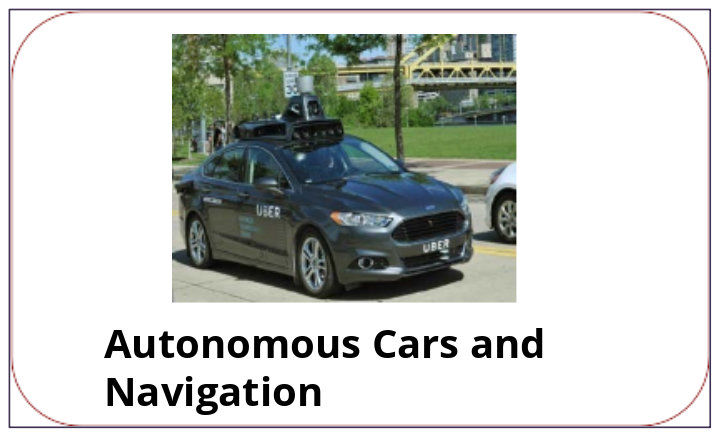
\includegraphics[width=0.98\textwidth, height=0.5\textheight]{Images/demystifying_car.png} \end{flushright}}
        \end{column}

	\begin{column}{0.5\textwidth}
		\only<3>{\begin{flushleft}  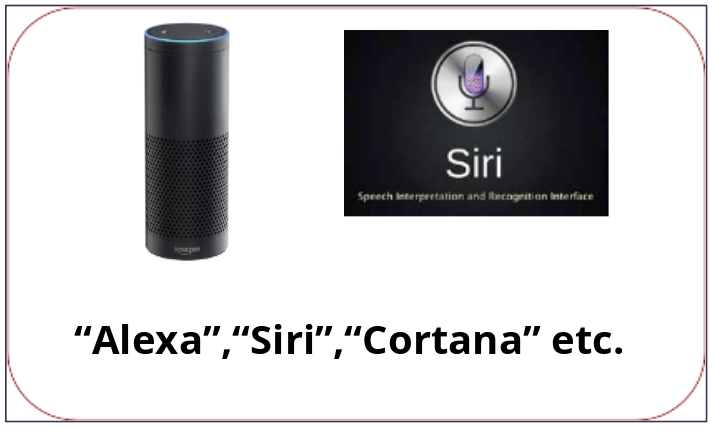
\includegraphics[width=0.98\textwidth, height=0.5\textheight]{Images/demystifying_siri.png}\end{flushleft}}	
	\end{column}

\end{columns}

\end{frame}

% Frame No : 3
\begin{frame}{AI and ML at Work}

	\begin{columns}

        \begin{column}{0.5\textwidth}
		\only<2->{ \begin{flushright} 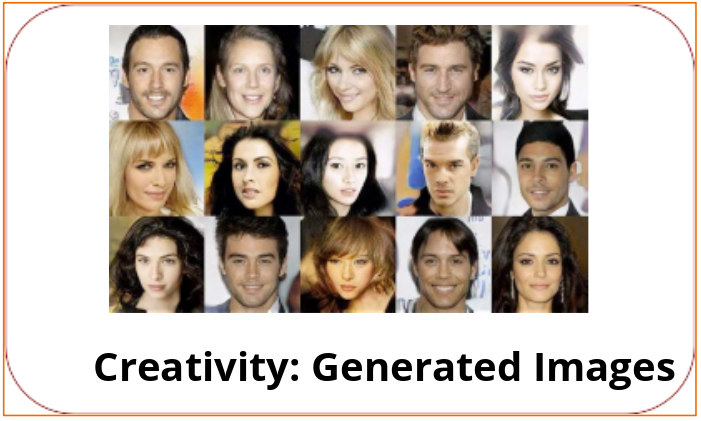
\includegraphics[width=0.98\textwidth, height=0.5\textheight]{Images/demystifying_creativity.png}\end{flushright}}
        \end{column}

        \begin{column}{0.5\textwidth}
		\only<3>{\begin{flushleft}  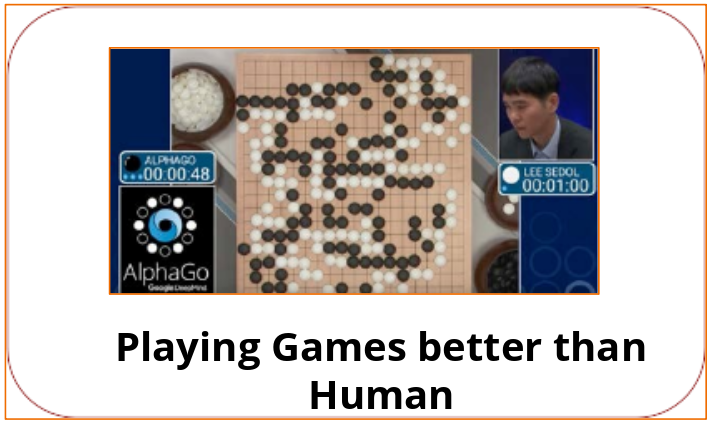
\includegraphics[width=0.98\textwidth, height=0.5\textheight]{Images/demystifying_games.png}\end{flushleft}}
        \end{column}

\end{columns}

\end{frame}


% Frame No : 4
\begin{frame}{Modern AI: End 2 End Driving}
	\vspace{-0.3cm}
	
	\only<2->{\centering 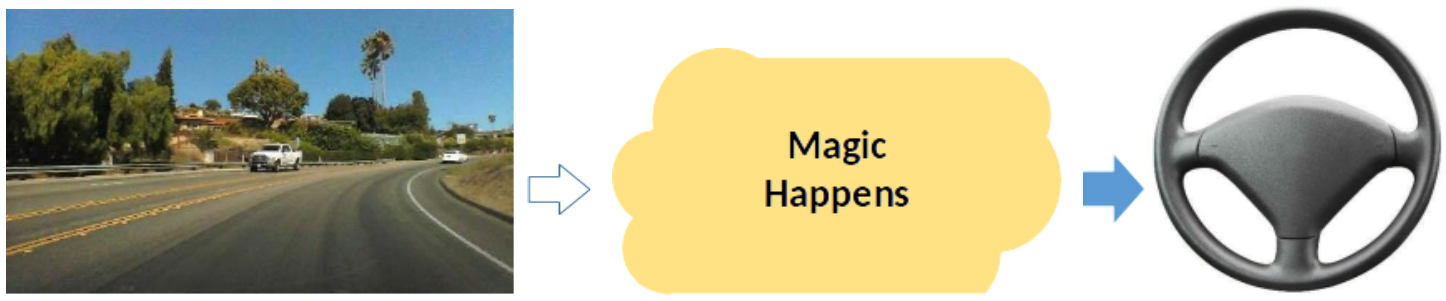
\includegraphics[width=0.8\textwidth, height=0.3\textheight]{Images/demystifying_magic.png} \\[100pt]}
	\only<3>{\vspace{-2.8cm} \centering 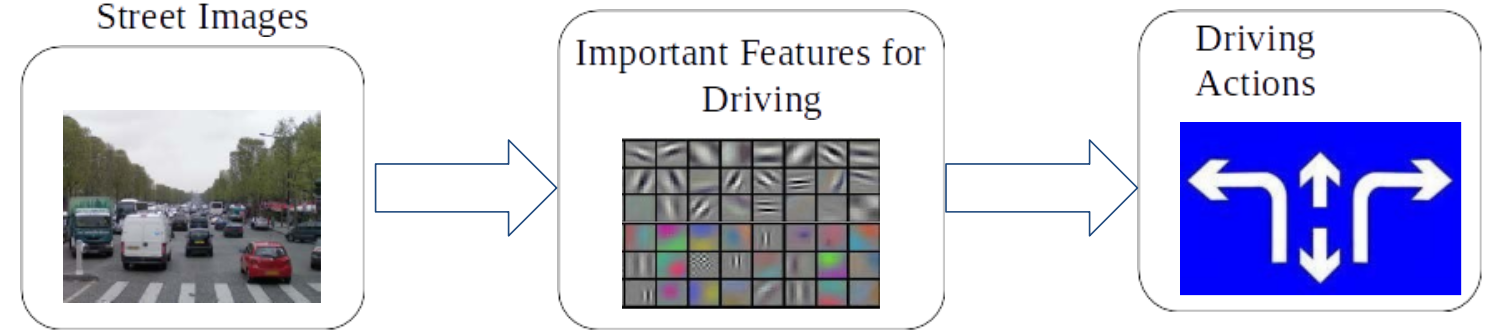
\includegraphics[width=0.8\textwidth, height=0.3\textheight]{Images/demystifying_street.png}}
	\transfade<3>
\end{frame}

% Frame No : 5
\begin{frame}{What is Modern AI and ML}
	\centering{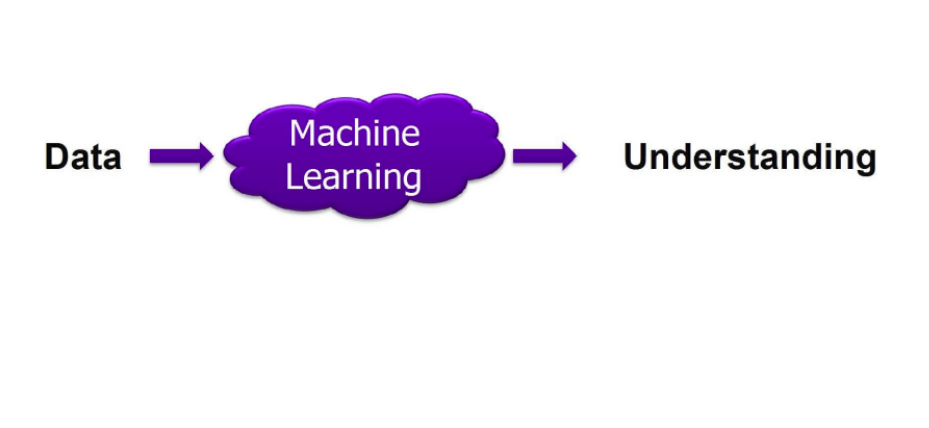
\includegraphics[width=15cm,height=8cm]{Images/WhatAIML.png}}
\end{frame}

%Frame No: 6
\begin{frame}{Modern “AI”}
	\only<1>{\centering 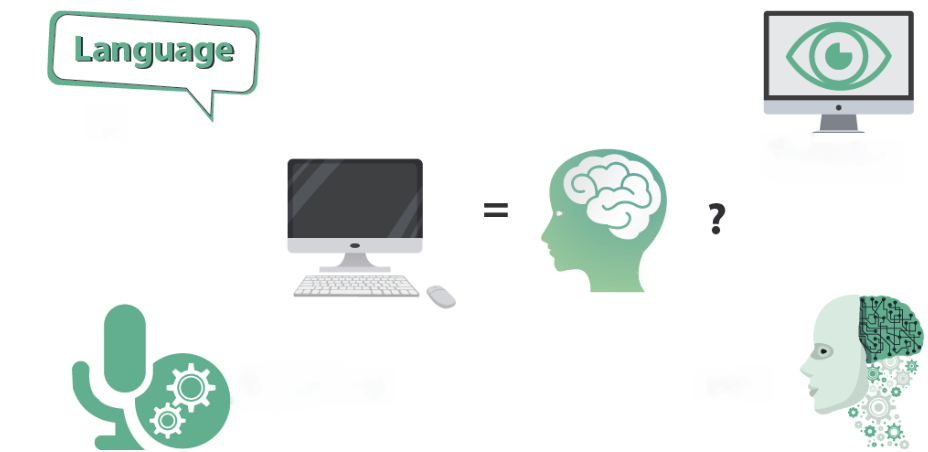
\includegraphics[width=0.75\textwidth, height=0.41\textwidth]{Images/demystifying_modernAI.png}}
	\only<2>{\hspace{-0.17cm}\centering 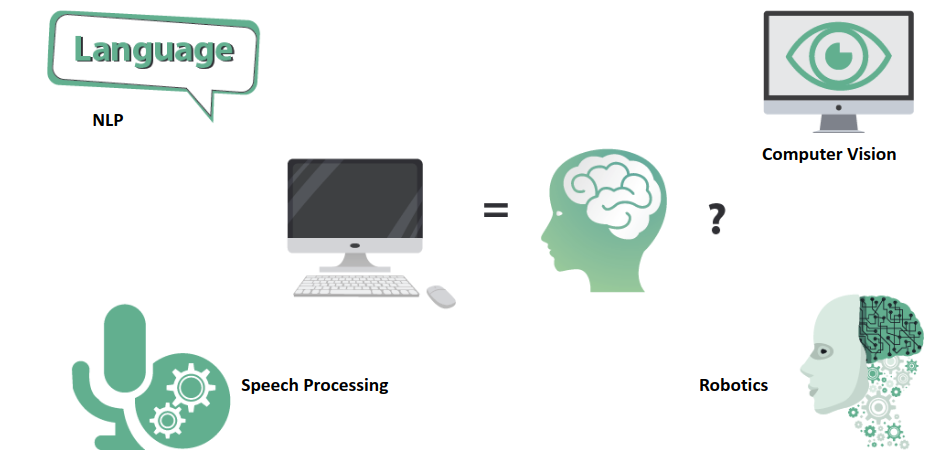
\includegraphics[width=0.75\textwidth, height=0.41\textwidth]{Images/demystifying_modernAI1.png}}
\end{frame}

%Frame No : 7
{\1
\begin{frame}
	\title{	A Simplified View }
	\subtitle{Demystifying ML}
	\titlepage
\end{frame}}

% Frame No: 8
\begin{frame}{A Simple Question }
\begin{itemize}
\item<2-> \alert{1, 3, 5, 7, 9,...What is the next number?}
\item<3-> \textcolor{black}{Ans: 11	Odd numbers} \only<4->{ \alert{$2x+1$}}

\vspace{1cm}
	
\item<5-> \alert{1, 3, 9, 19, 33, ... What is the next number?}
\item<6-> \textcolor{black}{Ans: 51} \only<7->{\alert{$2x^2+1$}}
\end{itemize}
\end{frame}

% Frame No: 9
\begin{frame}{A Simple Question}
\begin{itemize}
\item<2-> \alert{How do we solve such problems?}
\end{itemize}
\begin{itemize}
\item<3-> \textcolor{black}{Find a pattern from the examples}
\setbeamertemplate{itemize items}[circle]
  \begin{itemize}
  \item<3-> \textcolor{black}{(function \alert{$f(x)=2x^2+1$} or model the data)}
\end{itemize}
\end{itemize}
\begin{itemize}
\item<4-> \textcolor{black}{Use it to predict the next number (or solve the  problem)}
\item<5-> \alert{How do we design a computational procedure?}
\end{itemize}
\end{frame}


% Frame No: 10
\begin{frame}{A Simplified View of ML}
\begin{figure}
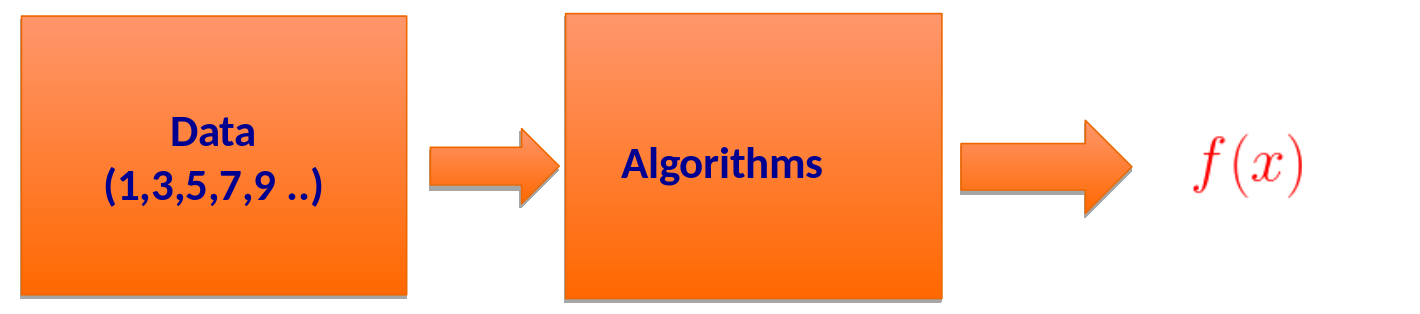
\includegraphics[width=\textwidth,height=0.35\textheight]{Images/demystifying_algorithms.png}
\end{figure}
	\begin{columns}
		\column{0.65\textwidth}
		\column{0.35\textwidth}
	Eg: 
		\\\textsl{int} $function(int x[]) \{ $ \\
	... \\
	\}
	
	\end{columns}
\end{frame}

% Frame No: 11
\begin{frame}{A Simple Question (cont.)}
\begin{itemize}
	\item<2-> \textcolor{black}{We know: 1, 3, 9, 19, 33, ..... What is the next number?\\ \textcolor{white}{.\\} Ans: 51 \vspace{25pt}}     \only<3->{\alert{$2x^2+1$}}
\item<4-> \textcolor{black}{ 0.99, 3.02, 9.00, 18.98, 33.01, ... What next?} 
\end{itemize}
\end{frame}

% Frame No: 12
\begin{frame}{A Simple Question (cont.)}
\begin{columns}
\column{0.6\textwidth}
\begin{overlayarea}{7cm}{5cm}
	\only<2->{\textcolor{black}{Consider a series of 2D points }}
\begin{itemize}
\item<2-> \textcolor{black}{(1,3), (2,6), (3,9), (4,12), ....}
\item<2-> \textcolor{blue}{\vspace{20pt}What is the next point?}
\item<4-> \textcolor{black}{\alert{$(x,3x)$ or}}
%\setbeamertemplate{itemize items}[circle]
  \begin{itemize}
  \item Function: \alert{y=f(x)=3x}
\end{itemize}
\end{itemize}
\end{overlayarea}
\column{0.4\textwidth}
\begin{overlayarea}{6.5cm}{4cm}
	\only<3>{\hspace{-2cm}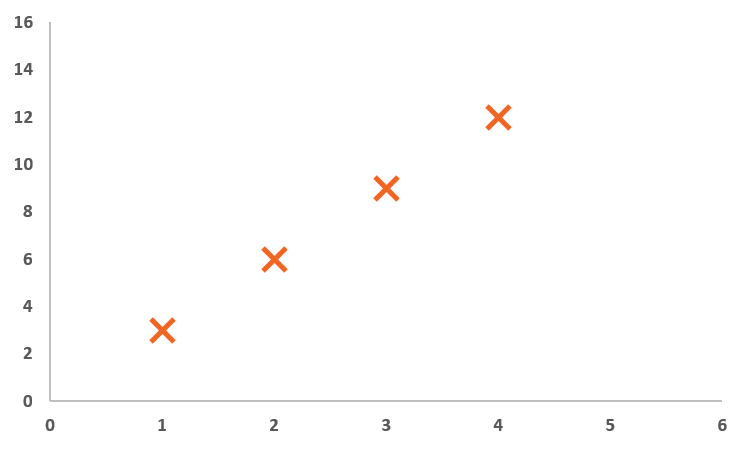
\includegraphics[width=6.5cm, height=4cm]{Images/demystifying_2dpoints.png}}
	\only<4>{\hspace{-2cm}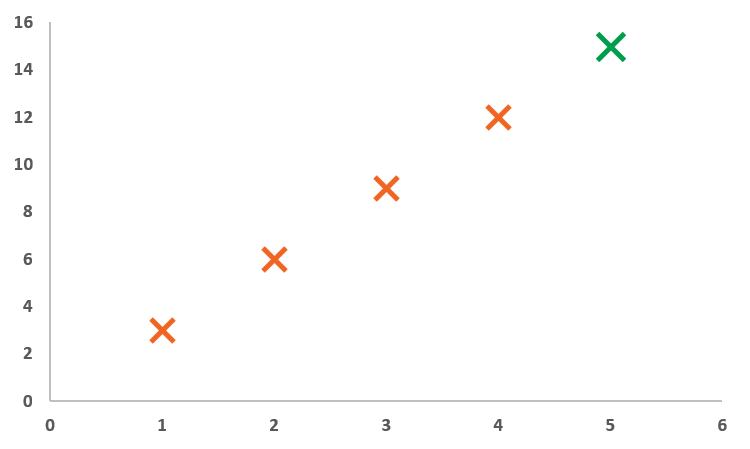
\includegraphics[width=6.5cm, height=4cm]{Images/demystifying_2dpoints_1.png}}
	\end{overlayarea}
\end{columns}
\end{frame}

% Frame No: 13
\begin{frame}{What Makes it Difficult?}
\begin{itemize}
\item<2-> \textcolor{blue}{When numbers are “uncertain”}
\setbeamertemplate{itemize items}[circle]
\begin{itemize}
\item<2-> \textcolor{black}{Noise in measurements}
\item<2-> \textcolor{black}{\vspace{5pt}Missing values}
\end{itemize}
\item<3-> \textcolor{blue}{When numbers are not just “simple numbers”}
\setbeamertemplate{itemize items}[circle]
\begin{itemize}
  \item<3-> \textcolor{black}{2D points, 3D points}
  \item<3-> \textcolor{black}{100 Dimensional points}
\end{itemize}
\end{itemize}
\end{frame}

% Frame No: 14
\begin{frame}{What Makes it Difficult?}
\begin{itemize}
\item<2> \textcolor{blue}{When the function is complex or function nature  is unknown}
\setbeamertemplate{itemize items}[circle]
  \begin{itemize}
  \item<2> \textcolor{black}{Simple linear functions are easy to guess.}\\
  \setbeamertemplate{itemize items}[circle]
\begin{itemize}
\item<2> Eg. \textcolor{red}{\vspace{5pt}$f(x) = \omega_{1}x+\omega_{2}$}
\end{itemize}
\end{itemize}
\begin{itemize}
	\item<2> \textcolor{black}{Finding \enquote{best} parameters/coefficients can be hard.}
\setbeamertemplate{itemize items}[circle]
  \begin{itemize}
	  \item<2> What is the best \textcolor{red}{\enquote{$\omega$}}that suits the data?
  \end{itemize}
\end{itemize}
\end{itemize}
\end{frame}

%Frame  No: 15
\begin{frame}{More Examples}
\begin{itemize}
\item<2-> \textcolor{black}{Given a set of numbers \{7,26,17,11,25,32,5,8,92\},\\
  partition into two sets: (Unsupervised Learning) \vspace{10pt}}
\item<3-> \textcolor{black}{Odd (7,17,11,25,5) and \vspace{10pt} Even (26,32,8,92)} 
\item<4-> \alert{Why this? Why not single and two \vspace{10pt} digit?}
\item<5-> \alert{Both mine and your solutions can be right?}
\end{itemize}
\end{frame}

% Frame No: 16
\begin{frame}{More Examples }
\begin{itemize}
\item<1-> \textcolor{blue}{ Given a set of male people with and without  anemia,\\         their hemoglobin levels are: (Supervised  Learning)\vspace{5pt} }
\setbeamertemplate{itemize items}[circle]
  \begin{itemize}
  \item<2-> \textcolor{black}{Positive cases: \{8.5, 9.2, 7.4, 7.8\}}
  \item<3-> \textcolor{black}{Negative cases: \{15.0, 14.9, 14.2,13.8\}}
  \item<4-> \textcolor{blue}{Does a patient with 7.7 have anemia?}
  \item<5-> \textcolor{black}{Classification is simple: “anemia if\alert{ $f(x)<10$}”}
  \item<6-> \textcolor{black}{Why 10? Why not 12?}
  \item<7-> \textcolor{black}{Multiple solutions. Both works well now. Future?} 
  \end{itemize}
\end{itemize}
\end{frame}

% Frame No: 17
\begin{frame}{Closer Look..}
\begin{itemize}
	\item<2-> {\alert{Who gives samples/examples?}}
\setbeamertemplate{itemize items}[circle]
\begin{itemize}
  \item<2-> \textcolor{black}{The Data}
  \item<2-> \textcolor{black}{Data + interpretations \alert{$(x,y)$} = (sample, label)}
\setbeamertemplate{itemize items}[circle]
\begin{itemize} 
 \item<2-> \textcolor{black}{Interpretations are the “supervisory signals”}
\end{itemize}
\end{itemize}
\end{itemize}
\begin{itemize}
\item<3-> \alert{Who gives functional form}
\setbeamertemplate{itemize items}[circle]
\begin{itemize}
  \item<3-> \textcolor{black}{Most problems need complex functions}\\
        (Note that simple “Linear” solutions are also good in many cases.)
\end{itemize}
\end{itemize}
\end{frame}

%Frame NO: 18
\begin{frame}{Closer Look..}
\begin{itemize}
\item<2-> {\textcolor{red}{How to find the “optimal” parameters?}}
\setbeamertemplate{itemize items}[circle]
\begin{itemize}
  \item<2-> \textcolor{black}{Optimization problem}\\
	  \begin{itemize}
		  \item \textcolor{black}{Find the best \alert{“$\omega”$} (coefficients) for a given data/problem?}
	  \end{itemize}
  \item<2-> \textcolor{black}{Training}
  \item<2-> \textcolor{black}{Computing}
\end{itemize}
\end{itemize}

\begin{itemize}
\item<3-> {\alert{How do we expect that it will work well in the  future?}}
\end{itemize}
\end{frame}





% Frame No: 19
\begin{frame}[t]{“Classification”:A Popular Problem}
	\vspace{-0.7cm}
	\begin{itemize}
\item \alert{Example:}
\setbeamertemplate{itemize items}[circle]
\begin{itemize}
  \item \textcolor{black}{Given medical records, predict presence of Malaria}
\end{itemize}
\end{itemize}
\begin{itemize}
\item \textcolor{black}{\alert{Data:}  A set of samples \{ X \} labeled by experts.}
\item \alert{Performance:} \textcolor{black}{Predict accurately on unseen data}
\end{itemize}
	\begin{columns}
		\column{0.01\textwidth}
		\column{0.5\textwidth}
	\begin{itemize}
		\item \hspace{4pt}{\textcolor{black}{\{0,1\} classification}}
		\begin{itemize}
\setbeamertemplate{itemize items}[circle]
		 \item \hspace{2pt}{\textcolor{black}{“Yes” or “No”}}
                 \item \hspace{2pt}{\textcolor{black}{Yes if \alert{$f(x)>0$}}}
\end{itemize}
\item \alert{Multiclass classification}
\item \alert{Many more variants}
\end{itemize}
		\column{0.49\textwidth}
		 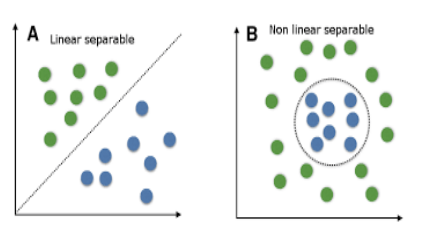
\includegraphics[width=6cm ,height=3.5cm]{Images/demystifying_linear.png}
	\end{columns}
\end{frame}

% Frame No: 20
\begin{frame}{Problem Space}
\begin{itemize}
	\item<2-> \alert{Feature Extraction:} Find $\alert{x}$ corresponding to an  entity/item (such as an image, web page, ECG  etc.). Let us denote by \alert{I}
	\item<3-> \alert{Classification}: Find a parameterized function which can make the right predictions. \\ We denote the function by \alert{\textit{$f$}} \\ We denote the predictions by \alert{\textit{$y$}}

\item<4-> \alert{End to End:} Can we learn \alert{$y$} directly from \alert{$I$}

\end{itemize}
\end{frame}

% Frame No: 21
\begin{frame}{Traditional Programming}
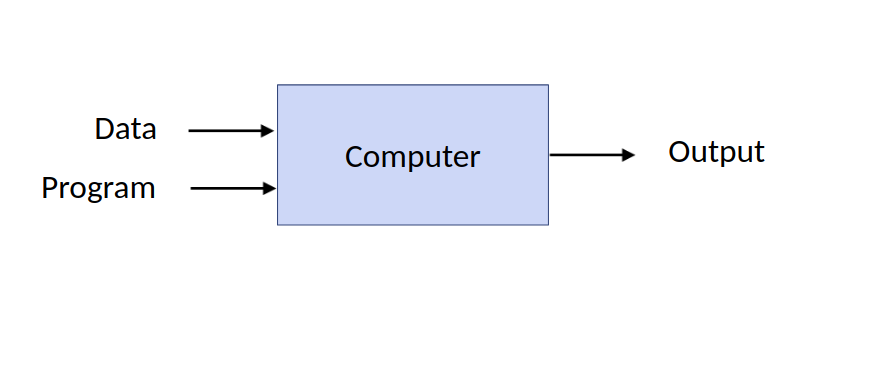
\includegraphics[width=\textwidth,height=0.65\textheight]{Images/demystifying_TP.png}
\end{frame}

% Frame No: 22
\begin{frame}{Machine Learning}
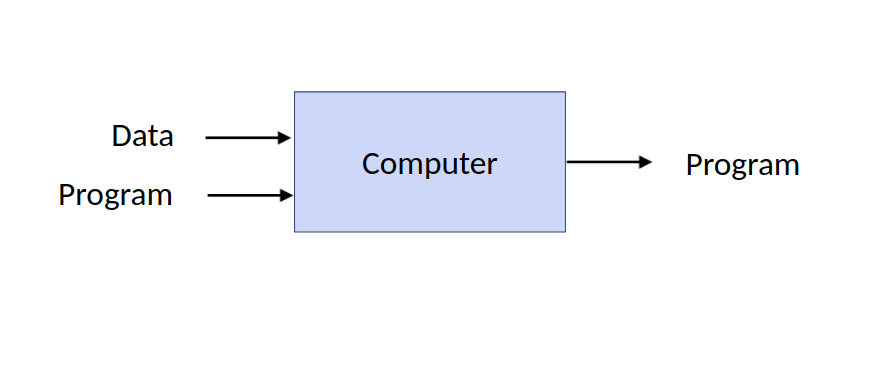
\includegraphics[width=\textwidth,height=0.65\textheight]{Images/demystifying_ML.png}
\end{frame}

% Frame No: 23
\begin{frame}{Machine Learning}
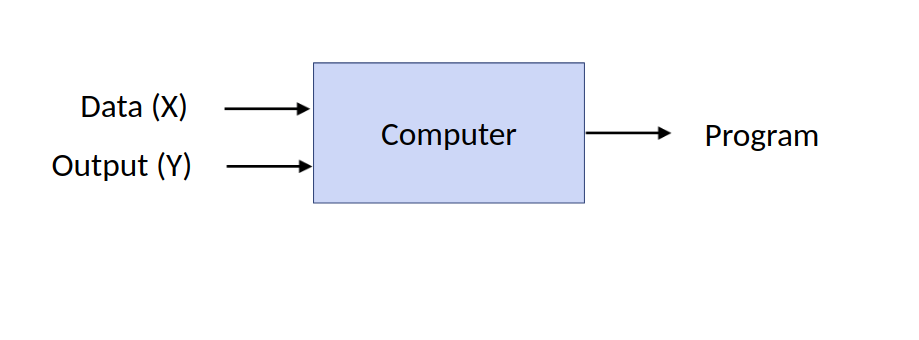
\includegraphics[width=\textwidth,height=0.65\textheight]{Images/demystifying_ML1.png}
\end{frame}

% Frame No: 24
{\1
\begin{frame}
	\title{Thanks!!}
	\subtitle{Questions?}
	\titlepage
\end{frame}
}


%\begin{frame}
%\footnotetext{Last updated version: 0.0\\
%            \textcolor{white}{---} Date: 12/04/2019 5:02p.m.}

%\end{frame}

\end{document}



